\documentclass[12pt]{article}
\usepackage[utf8]{inputenc}
\usepackage[spanish]{babel}
\usepackage[none]{hyphenat} % no cortar las palabras
\usepackage[margin=25mm]{geometry}
    \hyphenation{thatshouldnot}
\usepackage{graphicx}
    \graphicspath{{images/}}
\usepackage{tikz}
    \usetikzlibrary{shapes,arrows,positioning}
\usepackage{float}
\usepackage{listings} % for codeblocks
\renewcommand{\lstlistingname}{Código}% Listing -> Algorithm
\usepackage{parskip}

\begin{document}

\begin{titlepage}
    \centering
    {\scshape\LARGE Universidad Católica de Santa María \par}
    \vspace{3em}
    \includegraphics[width=0.25\textwidth]{$HOME/.config/latex/images/Escudo-UCSM.png}\par\vspace{3em}
    \vspace{1cm}
    {\scshape\Large Escuela Profesional de Ingeniería Electrónica \par}
    \vspace{1.5cm}
    {\huge\bfseries Informe 4NEC2\par}   % título del proyecto
    \vspace{2cm}
    \large
    {\bfseries Curso:} Software de Telecomunicaciones\par
    {\bfseries Alumno:} Luis Orlando Figueroa Morales\par
    {\bfseries Docente:} Ing. Mario Urrutia Espinoza 

    \vfill

    {\small Arequipa - 2021\par}
\end{titlepage}

\section{Introducción}

4NEC2 es un programa libre para modelizar antenas. Además de ser una
herramienta potente para crear, ver optimizar y probar estructura de antenas en
2D y 3D que tambíen genera, muestra y compara campos cercanos y lejanos de
radiación.

Algunas de las herramientas que vienen en 4NEC2 son el Optimizer y Sweeper con
el cual se pueden hacer optimizaciones en la antena cuando se ejecutan barridos
de frequencia haciendo que se generen gráficos de líneas de impedancia, ROE,
ganancia, relación F/B de estilo lineal y logarítmico. Haciendo el Sweeper (o
barrido) se puede mostrar de manera gráfica.

\begin{figure}[H]
\centering
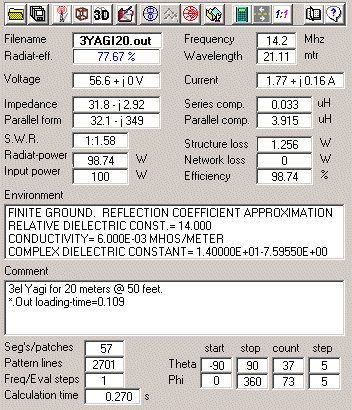
\includegraphics[width=.4\linewidth]{images/image002.png}
\caption{Ventana principal de 4NEC2.}
\end{figure}

\section{Características}

Algunas de las características que este software nos detalla en su
documentación (https://www.qsl.net/4nec2/) son:

\begin{itemize}
\item Las gráficas en 2D y 3D de visualización de estructuras geométricas.
\item Opción para arrastrar y soltar para poder modelar antenas.
\item Visualización interactiva de la Carta de Smith para barridos de
frequencia.
\item Archivo de ayuda de manera contextual.
\end{itemize}


\end{document}
